 %\documentclass[preprint,12pt]{elsarticle}

%% Use the options 1p,twocolumn; 3p; 3p,twocolumn; 5p; or 5p,twocolumn
%% for a journal layout:
%%  \documentclass[final,1p,times]{elsarticle}
%% \documentclass[final,1p,times,twocolumn]{elsarticle}
%% \documentclass[final,3p,times]{elsarticle}
%% \documentclass[final,3p,times,twocolumn]{elsarticle}
%\documentclass[final,5p,times]{elsarticle}
\documentclass[final,5p,times,twocolumn]{elsarticle}

\newcommand{\note}[2][inline]{\todo[color=red!30,#1]{\small\sf #2}}

%% if you use PostScript figures in your article
%% use the graphics package for simple commands
%% \usepackage{graphics}
%% or use the graphicx package for more complicated commands
%% \usepackage{graphicx}
%% or use the epsfig package if you prefer to use the old commands
%% \usepackage{epsfig}

%% The amssymb package provides various useful mathematical symbols
\usepackage{rotating,todonotes, xspace}
\usepackage{amssymb}
\usepackage[section]{placeins}
\usepackage{makeidx}  % allows for indexgeneration
\usepackage{algorithm}
\usepackage{algpseudocode}
\usepackage{graphicx}
\usepackage{float}
\usepackage{subcaption}
\captionsetup{compatibility=false}
\usepackage{wrapfig}
\usepackage{array}
\usepackage{multicol}
\usepackage{hyperref}
\usepackage{enumitem}

% The amsthm package provides extended theorem environments
%% \usepackage{amsthm}


\journal{Future Generation of Computer Systems}

\begin{document}

\begin{frontmatter}

%Should change the tilte to something better
\title{Using Imbalance Metrics to Optimize Task Clustering in Scientific Workflow Executions}


\author[isi]{Weiwei Chen\corref{cor1}}
\ead{weiweich@acm.org}

\author[isi]{Rafael Ferreira da Silva}
\ead{rafsilva@isi.edu}

\author[isi]{Ewa Deelman}
\ead{deelman@isi.edu}

\author[man]{Rizos Sakellariou}
\ead{rizos@cs.man.ac.uk}

\cortext[cor1]{Corresponding address: USC Information Sciences Institute, 4676 Admiralty Way Ste 1001, Marina del Rey, CA, USA, 90292, Tel: +1 310 448-8408}


\address[isi]{University of Southern California, Information Sciences Institute, Marina del Rey, CA, USA}
\address[man]{University of Manchester, School of Computer Science, Manchester, U.K.}


\begin{abstract}
Scientific workflows can be composed of many fine computational granularity tasks. The runtime of these tasks may be shorter than the duration of system overheads, for example, when using multiple resources of a cloud infrastructure. Task clustering is a runtime optimization technique that merges multiple short running tasks into a single job such that the scheduling overhead is reduced and the overall runtime performance is improved. However, existing task clustering strategies only provide a coarse-grained approach that relies on an over-simplified workflow model. In this work, we examine the reasons that cause Runtime Imbalance and Dependency Imbalance in task clustering. Then, we propose quantitative metrics to evaluate the severity of the two imbalance problems. Furthermore, we propose a series of task balancing methods (horizontal and vertical) to address the load balance problem when performing task clustering for 5 widely used scientific workflows. Finally, we analyze the relationship between these metric values and the performance of these task balancing methods. A trace-based simulation shows our methods can significantly improve the runtime performance of workflow applications when compared to a baseline execution. We also compare the performance of our methods with two algorithms from the literature.

\end{abstract}

\begin{keyword}
Scientific workflows \sep Performance analysis \sep Scheduling \sep Workflow simulation \sep Task clustering \sep Load balancing
\end{keyword}

\end{frontmatter}


\section{Introduction}
\label{intro}
Many computational scientists develop and use large-scale, loosely-coupled applications that are often structured as scientific workflows. Although the majority of the tasks within these applications are often relatively short running (from a few seconds to a few minutes), in aggregate they represent a significant amount of computation and data~\cite{daSilva:2013:TFO:2534248.2534254,Juve2013}. When executing these applications in a multi-machine{, }distributed environment, such as the Grid or the Cloud, significant system overheads may exist and may slowdown the application {execution}~\cite{Chen2011}. To reduce the impact of such overheads, task clustering techniques~\cite{Muthuvelu:2005:DJG:1082290.1082297,4493929,Muthuvelu2010,Muthuvelu2013170,keat-2006,ang-2009,Liu2009,Singh:2008:WTC:1341811.1341822,Ferreira-granularity-2013} have been developed to group \emph{fine-grained} tasks into \emph{coarse-grained} tasks so that the number of computational activities is reduced and {so that }their computational granularity is increased{.  This reduced }the (mostly scheduling related) system overheads.
However, there are several challenges that have not yet been addressed.

A scientific workflow is typically represented as a directed acyclic graph (DAG). {The nodes represent computations and the edges describe data and control dependencies between them. }Tasks within a level (or depth within a workflow DAG) may have different runtimes. {Proposed task clustering techniques that merge  }tasks within a level without considering the runtime variance may cause load imbalance, i.e., some clustered jobs may be composed of short running tasks while others of long running tasks. This imbalance delays the release of tasks from the next level of the workflow, penalizing the workflow execution with an overhead produced by the use of inappropriate task clustering strategies~\cite{Chen2013}.
A common technique to handle load imbalance is overdecomposition~\cite{Lifflander}.
This method decomposes computational work into \emph{medium-grained} balanced tasks. Each task is coarse-grained enough to enable efficient execution and reduce scheduling overheads, while being fine-grained enough to expose significantly higher application-level parallelism than what is offered by the hardware. 

Data dependencies between workflow tasks play an important role when clustering tasks within a level. A data dependency means that there is a data transfer between two tasks (output data for one and input data for the other). Grouping tasks without considering these dependencies may lead to data locality problems{, }where output data produced by parent tasks are poorly distributed. As a result, data transfer times and failure probabilities increase.
Therefore, we claim that data dependencies of subsequent tasks should be considered.

We generalize these two challenges (Runtime Imbalance and Dependency Imbalance) to the general task clustering load balance problem. We introduce a series of balancing methods to address these challenges. However, there is a tradeoff between runtime and data dependency balancing. For instance, balancing runtime may aggravate the Dependency Imbalance problem, and vice versa. Therefore, we propose a series of quantitative metrics that reflect the internal structure (in terms of task runtimes and dependencies) of the workflow and use them as a criterion to select and balance {the } solutions.

In particular, we provide a novel approach to capture {the imbalance } metrics. Traditionally, there are two approaches to improve the performance of task clustering. The first one is a top-down approach \cite{6217508} that represents the clustering problem as a global optimization problem and aims to minimize the overall workflow execution time. However, the complexity of solving such an optimization problem does not scale well since most solutions are based on genetic algorithms. The second one is a bottom-up approach~\cite{Muthuvelu:2005:DJG:1082290.1082297,Liu2009} that only examines free tasks to be merged and optimizes the clustering results locally. In contrast, our work extends these approaches to consider the neighboring tasks including siblings, parents, and children{, } because such a family of tasks has strong connections between them. 

The quantitative metrics and balancing methods were introduced and evaluated in~\cite{6683907} on {five }workflows. In this {paper}, we extend this previous work by studying:

\begin{itemize}[noitemsep,nolistsep]
	\item the performance gain of using our balancing methods over a baseline execution on a larger set of workflows;
	\item the performance gain over two additional task clustering methods described in the literature~\cite{ang-2009,Liu2009};
	\item the performance impact of the variation of the average data size and number of resources;
	\item the performance impact of combining our balancing methods with vertical clustering.
\end{itemize}

The rest of {the paper } is organized as follows. Section~\ref{sec:related-work} gives an overview of the related work. Section~\ref{sec:model} presents our workflow and execution environment models. Section~\ref{sec:imbalance} details our heuristics and algorithms for balancing. Section~\ref{sec:experiments} reports experiments and results, and the {paper } closes with a discussion and conclusions.

% Section
\section{Related Work}
\label{sec:related-work}

{System }overhead analysis~\cite{Ostberg2011, Prodan2008} is a topic of great interest in the {distributed computing } community. Stratan et al.~\cite{Stratan2008} evaluate in a real-world environment Grid workflow engines including DAGMan/Condor and Karajan/Globus. Their methodology focuses on five system characteristics: overhead, raw performance, stability, scalability, and reliability. They {point } out that {resource consumption in head nodes }should not be {ignored } and {that } the main bottleneck in a busy system is often the head node. Prodan et al.~\cite{Prodan2008} offered a complete Grid workflow overhead classification and a systematic measurement of overheads. In Chen et al.~\cite{Chen2011}, we extended~\cite{Prodan2008} by providing a measurement of major overheads imposed by workflow management systems and execution environments and analyzed how existing optimization techniques improve {the workflow }runtime by reducing or overlapping overheads. The prevalent existence of system overheads is an important reason why task clustering provides significant performance improvement for workflow-based applications. In this chapter, we aim to further improve the performance of task clustering under imbalanced load. 

The low performance of \emph{fine-grained} tasks is a common problem in widely distributed platforms where the scheduling overhead and queuing times at resources are high, such as Grid and Cloud systems. Several works have addressed the control of task granularity of bags of tasks. For instance, Muthuvelu et al.~\cite{Muthuvelu:2005:DJG:1082290.1082297} proposed a clustering algorithm that groups bags of tasks based on their runtime---tasks are grouped up to the resource capacity. Later, they extended their work~\cite{4493929} to determine task granularity based on task file size, CPU time, and resource constraints. Recently, they proposed an online scheduling algorithm~\cite{Muthuvelu2010,Muthuvelu2013170} that groups tasks based on resource network utilization, user's budget, and application deadline. Ng et al.~\cite{keat-2006} and Ang et al.~\cite{ang-2009} introduced bandwidth in the scheduling framework to enhance the performance of task scheduling. Longer tasks are assigned to resources with better bandwidth. Liu and Liao~\cite{Liu2009} proposed an adaptive fine-grained job scheduling algorithm to group fine-grained tasks according to processing capacity and bandwidth of the current available resources. Although these techniques significantly reduce the impact of scheduling and queuing time overhead, they {do } not consider data dependencies.

Task granularity control has also been addressed in scientific workflows. For instance, Singh et al.~\cite{Singh:2008:WTC:1341811.1341822} proposed level- and label-based clustering. In level-based clustering, tasks at the same level {of the workflow }can be clustered together. The number of clusters or tasks per cluster are specified by the user. In the label-based clustering {method}, the user labels tasks that should be clustered together. Although their work considers data dependencies between workflow levels, it is done manually by the users, which is prone to errors {and it is not scalable}. Recently, Ferreira da Silva et al.~\cite{Ferreira-granularity-2013,FerreiradaSilva-CCPE-2014} proposed task grouping and ungrouping algorithms to control workflow task granularity in a non-clairvoyant and online context, where none or few characteristics about the application or resources are known in advance. Their work significantly reduced scheduling and queuing time overheads, but did not consider data dependencies.

A plethora of balanced scheduling algorithms have been developed in the networking and operating system domains. Many of these schedulers have been extended to the hierarchical setting. Lifflander et al.~\cite{Lifflander} proposed to use work stealing and a hierarchical persistence-based rebalancing algorithm to address the imbalance problem in scheduling. Zheng et al.~\cite{Zheng} presented an automatic hierarchical load balancing method that overcomes the scalability challenges of centralized schemes and poor solutions of traditional distributed schemes. There are other scheduling algorithms~\cite{rizos2008} that indirectly achieve load balancing of workflows through makespan minimization. However, the benefit that can be achieved through traditional scheduling optimization is limited by its complexity. The performance gain of task clustering is primarily determined by the ratio between system overheads and task runtime, which is more substantial in modern distributed systems such as Clouds and Grids. 

Workflow patterns~\cite{Yu2005a, Juve2013, Liu2008} are used to capture and abstract the common structure within a workflow and they give insights on designing new workflows and optimization methods. Yu and Buyya~\cite{Yu2005a} proposed a taxonomy that characterizes and classifies various approaches for building and executing workflows on Grids. They also provided a survey of several representative Grid workflow systems developed by various projects world-wide to demonstrate the comprehensiveness of the taxonomy. Juve et al.~\cite{Juve2013} provided a characterization of workflow from six scientific applications and obtained task-level performance metrics (I/O, CPU, and memory consumption). They also presented an execution profile for each workflow running at a typical scale and managed by the Pegasus workflow management system~\cite{Deelman2004, Deelman:2005:PFM:1239649.1239653, deelman2014pegasus}. Liu et al.~\cite{Liu2008} proposed a novel pattern based time-series forecasting strategy which utilizes a periodical sampling plan to build representative duration series. We illustrate the relationship between the workflow patterns (asymmetric or symmetric workflows) and the performance of our balancing algorithms. 

Some work in the literature has further attempted to define and model workflow characteristics with quantitative metrics. In~\cite{Ali2004}, the authors proposed a robustness metric for resource allocation in parallel and distributed systems and accordingly customized the definition of robustness. Tolosana et al.~\cite{Tolosana2011} defined a metric called Quality of Resilience to assess how resilient workflow enactment is likely to be in the presence of failures. Ma et al. ~\cite{Ma:2014:GDB:2560969.2561388} proposed a graph distance based metric for measuring the similarity between data oriented workflows with variable time constraints, where a formal structure called time dependency graph (TDG) is proposed and further used as representation model of workflows. Similarity comparison between two workflows can be reduced to computing the similarity between TDGs. In this work, we develop quantitative metrics to measure the severity of the imbalance problem in task clustering and then use the results to guide the selection of different task clustering methods.


% Section
\section{Related Work}
\label{sec:related-work}

\rev{System }overhead analysis~\cite{Ostberg2011, Prodan2008} is a topic of great interest in the \rev{distributed computing } community. Stratan et al.~\cite{Stratan2008} evaluate in a real-world environment Grid workflow engines including DAGMan/Condor and Karajan/Globus. Their methodology focuses on five system characteristics: overhead, raw performance, stability, scalability, and reliability. They \rev{point } out that \rev{resource consumption in head nodes }should not be \rev{ignored } and \rev{that } the main bottleneck in a busy system is often the head node. Prodan et al.~\cite{Prodan2008} offered a complete Grid workflow overhead classification and a systematic measurement of overheads. In Chen et al.~\cite{Chen2011}, we extended~\cite{Prodan2008} by providing a measurement of major overheads imposed by workflow management systems and execution environments and analyzed how existing optimization techniques improve \rev{the workflow }runtime by reducing or overlapping overheads. The prevalent existence of system overheads is an important reason why task clustering provides significant performance improvement for workflow-based applications. In this chapter, we aim to further improve the performance of task clustering under imbalanced load. 

The low performance of \emph{fine-grained} tasks is a common problem in widely distributed platforms where the scheduling overhead and queuing times at resources are high, such as Grid and Cloud systems. Several works have addressed the control of task granularity of bags of tasks. For instance, Muthuvelu et al.~\cite{Muthuvelu:2005:DJG:1082290.1082297} proposed a clustering algorithm that groups bags of tasks based on their runtime---tasks are grouped up to the resource capacity. Later, they extended their work~\cite{4493929} to determine task granularity based on task file size, CPU time, and resource constraints. Recently, they proposed an online scheduling algorithm~\cite{Muthuvelu2010,Muthuvelu2013170} that groups tasks based on resource network utilization, user's budget, and application deadline. Ng et al.~\cite{keat-2006} and Ang et al.~\cite{ang-2009} introduced bandwidth in the scheduling framework to enhance the performance of task scheduling. Longer tasks are assigned to resources with better bandwidth. Liu and Liao~\cite{Liu2009} proposed an adaptive fine-grained job scheduling algorithm to group fine-grained tasks according to processing capacity and bandwidth of the current available resources. Although these techniques significantly reduce the impact of scheduling and queuing time overhead, they \rev{do } not consider data dependencies.

Task granularity control has also been addressed in scientific workflows. For instance, Singh et al.~\cite{Singh:2008:WTC:1341811.1341822} proposed level- and label-based clustering. In level-based clustering, tasks at the same level \rev{of the workflow }can be clustered together. The number of clusters or tasks per cluster are specified by the user. In the label-based clustering \rev{method}, the user labels tasks that should be clustered together. Although their work considers data dependencies between workflow levels, it is done manually by the users, which is prone to errors \rev{and it is not scalable}. Recently, Ferreira da Silva et al.~\cite{Ferreira-granularity-2013,FerreiradaSilva-CCPE-2014} proposed task grouping and ungrouping algorithms to control workflow task granularity in a non-clairvoyant and online context, where none or few characteristics about the application or resources are known in advance. Their work significantly reduced scheduling and queuing time overheads, but did not consider data dependencies.

A plethora of balanced scheduling algorithms have been developed in the networking and operating system domains. Many of these schedulers have been extended to the hierarchical setting. Lifflander et al.~\cite{Lifflander} proposed to use work stealing and a hierarchical persistence-based rebalancing algorithm to address the imbalance problem in scheduling. Zheng et al.~\cite{Zheng} presented an automatic hierarchical load balancing method that overcomes the scalability challenges of centralized schemes and poor solutions of traditional distributed schemes. There are other scheduling algorithms~\cite{rizos2008} that indirectly achieve load balancing of workflows through makespan minimization. However, the benefit that can be achieved through traditional scheduling optimization is limited by its complexity. The performance gain of task clustering is primarily determined by the ratio between system overheads and task runtime, which is more substantial in modern distributed systems such as Clouds and Grids. 

Workflow patterns~\cite{Yu2005a, Juve2013, Liu2008} are used to capture and abstract the common structure within a workflow and they give insights on designing new workflows and optimization methods. Yu and Buyya~\cite{Yu2005a} proposed a taxonomy that characterizes and classifies various approaches for building and executing workflows on Grids. They also provided a survey of several representative Grid workflow systems developed by various projects world-wide to demonstrate the comprehensiveness of the taxonomy. Juve et al.~\cite{Juve2013} provided a characterization of workflow from \rev{six } scientific applications and obtained task-level performance metrics (I/O, CPU, and memory consumption). They also presented an execution profile for each workflow running at a typical scale and managed by the Pegasus workflow management system\rev{~\cite{Deelman2004, Deelman:2005:PFM:1239649.1239653, deelman2014pegasus}}. Liu et al.~\cite{Liu2008} proposed a novel pattern based time-series forecasting strategy which utilizes a periodical sampling plan to build representative duration series. We illustrate the relationship between the workflow patterns (asymmetric or symmetric workflows) and the performance of our balancing algorithms. 

Some work in the literature has further attempted to define and model workflow characteristics with quantitative metrics. In~\cite{Ali2004}, the authors proposed a robustness metric for resource allocation in parallel and distributed systems and accordingly customized the definition of robustness. Tolosana et al.~\cite{Tolosana2011} defined a metric called Quality of Resilience to assess how resilient workflow enactment is likely to be in the presence of failures. Ma et al. ~\cite{Ma:2014:GDB:2560969.2561388} proposed a graph distance based metric for measuring the similarity between data oriented workflows with variable time constraints, where a formal structure called time dependency graph (TDG) is proposed and further used as representation model of workflows. Similarity comparison between two workflows can be reduced to computing the similarity between TDGs. In this work, we \rev{develop quantitative metrics to measure the severity of the imbalance problem in task clustering and then use the results to guild the selection of different task clustering methods.}



\section{Model and Design}
\label{sec:model}


\begin{figure}[htb]
	\centering
	\includegraphics[width=0.7\linewidth]{figures/model/odag.pdf}
	\captionof{figure}{Extending DAG to o-DAG.}
	\label{fig:model_odag}
	\vspace{-10pt}
\end{figure}
A workflow is modeled as a Directed Acyclic Graph (DAG) as shown in Fig.~\ref{fig:model_odag} (Left). Each node in the DAG often represents a workflow job ($j$), and the edges represent dependencies between the jobs that constrain the order in which the jobs are executed. Dependencies typically represent data-flow dependencies in the application, where the output files produced by one job are used as inputs of another job. Each job is a single execution unit and it may contains one or multiple tasks, which is a program and a set of parameters that need to be executed. Fig.~\ref{fig:model_odag} (left) shows an illustration of a DAG composed by four jobs. This model fits several workflow management systems such as Pegasus~\cite{Deelman2005}, Askalon~\cite{Fahringer2005}, and Taverna~\cite{Oinn:2006:TLC:1148437.1148448}.

%Change it with job wrapper
Fig.~\ref{fig:model_system} shows a typical workflow execution environment. The submit host prepares a workflow for execution (clustering, mapping, etc.), and worker nodes, at an execution site, execute jobs individually. The main components are introduced below:

\begin{figure}[htb]
\centering
  \includegraphics[width=0.95\linewidth]{figures/model/execution.pdf}
  \caption{A workflow system model.}
  \label{fig:model_system}
  \vspace{-10pt}
\end{figure}

\paragraph{Workflow Mapper} generates an executable workflow based on an abstract workflow provided by the user or workflow composition system. It also restructures the workflow to optimize performance and adds tasks for data management and provenance information generation. In this work, workflow mapper is particularly used to merge small tasks together into a job such that system overheads are reduced, which is called Task Clustering. A job is a single execution unit in the workflow execution systems and it may contain one or more tasks.

\paragraph{Workflow Engine} executes jobs defined by the workflow in order of their dependencies. Only jobs that have all their parent jobs completed are submitted to the Job Scheduler. Workflow Engine relies on the resources (compute, storage, and network) defined in the executable workflow to perform the necessary actions. The time period when a job is free (all of its parents have completed successfully) to when it is submitted to the job scheduler is denoted the workflow engine delay. The workflow engine delay is usually configured by users to assure that the entire workflow scheduling and execution system is not overloaded. 

\paragraph{Job Wrapper} extracts tasks from clustered jobs and executes them at the worker nodes. The clustering delay is the elapsed time on the extraction process.



\paragraph{Job Scheduler and Local Queue} manage individual workflow jobs and supervise their execution on local and remote resources. The time period when a job is submitted to the job scheduler to when the job starts its execution in a worker node is denoted the queue delay. It reflects both the efficiency of the job scheduler and the resource availability. 


\begin{figure}[h!]
	\centering
    \includegraphics[width=0.5\textwidth]{figures/model/overhead.pdf}
    \caption{Workflow Events}
    \label{fig:model_overhead}
\end{figure}



The execution of a job is comprised of a series of events as shown in Fig.~\ref{fig:model_overhead} and they are defined as:

\begin{enumerate}
\item Job Release is defined as the time when the workflow engine identifies that a job is ready to be submitted (when its parents have successfully completed). 
\item Job Submit is defined as the time when the workflow engine submits a job to the local queue. 
\item Job Execute is defined as the time when the workflow engine sees a job is being executed. 
\item Task Execute is defined as the time when the job wrapper sees a task is being executed. 
\item Pre/Postscript Start is defined as the time when the workflow engine starts to execute a pre/postscript. 
\item Pre/Postscript Terminate is defined as the time when the pre/postscript returns a status code (success or failure). 
\end{enumerate}

Fig.~\ref{fig:model_overhead} shows a typical timeline of overheads and runtime in a compute job. We do not specify the data transfer delay in this timeline because data transfer is handled by data transfer jobs (stage-in and stage-out jobs). 

As shown in our prior work \cite{Chen2011}, we have classified workflow overheads into four categories as follows. 
\begin{enumerate}

\item{Workflow Engine Delay} measures the time between when the last parent job of a job completes and the time when the job gets submitted to the local queue. The completion time of the last parent job means this job is released to the ready queue and is waiting for resources to be assigned to it. The workflow engine delay reflects the efficiency of a workflow engine (i.e., DAGMan~\cite{DAGMan}). 

\item{Queue Delay} is defined as the time between the submission of a job by the workflow engine to the local queue and the time the local scheduler sees the job running. This overhead reflects the efficiency of the local workflow scheduler (e.g. Condor \cite{Frey2002}) to execute a job and the availability of resources for the execution of this job. 

\item{Pre/Postscript Delay } is the time taken to execute a lightweight script under some execution systems before/after the execution of a job. For example, prescripts prepare working environment before the execution of a job starts and postscripts examine the status code of a job after the computational part of this job is done.

\item{Clustering Delay} measures the difference between the sum of the actual task runtime and the job runtime seen by the job wrapper. The cause of Clustering Delay is usually because we use a job wrapper in worker nodes to execute a clustered job that requires some delay to extract the list of tasks. 

\end{enumerate}

The overhead aware DAG model (o-DAG) we use in this work is an extension of the traditional DAG model. System overheads play an important role in workflow execution and constitute a major part of the overall runtime when jobs are poorly mapped to resources. Fig.~\ref{fig:model_odag} shows how we augment a DAG to be an o-DAG with the capability to represent system overheads ($s$) such as workflow engine delay and queue delay.  In summary, an o-DAG representation allows the specification of high level system overhead details, which is more suitable for the study of overhead aware scheduling. 


\section{Imbalance Metrics}
\label{sec:imbalance}

%Need to fix this
With an o-DAG model, we can explicitly express the process of task clustering. For instance, in Fig. 3, two tasks t1 and t2, without data dependency between them, are merged into a clustered job j1. A job j is a single execution unit composed by one or multiple task(s). Job wrappers are commonly used to execute clustered jobs, but they add a overhead denoted the clustering delay c. Clustering delay measures the difference between the sum of the actual task runtimes and the job runtime seen by the job scheduler. After horizontal clustering, t1 and t2 in j1 can be executed in sequence or in parallel, if supported. In this paper, we consider sequential executions only. Given a single resource, the overall runtime for the workflow in Fig. 3 (left) is runtime1 = s1 +t1 +s2 +t2 , and the overall runtime for the clustered workflow in Fig. 3 (right) is runtime2 = s1 + c1 + t1 + t2. runtime1 > runtime2 as long as c1 < s2, which is the case of many distributed systems since the clustering delay within an execution node is usually shorter than the scheduling overhead across different execution nodes.
Fig 3 shows a typical example of a Horizontal Clustering. 

Fig. 3: An Example of Task Clustering.

(HC) technique that groups tasks at the same horizontal level. In our work, we define the level of a task as the longest depth from the root task to this task (Depth First Search) because the longest depth controls the final release of this task.


%Although the majority of the tasks within these applications are often relatively short running (from a few seconds to a few minutes), in aggregate they represent a significant amount of computation and data~\cite{LIGO}. When executing these applications on a multi-machine distributed environment, such as the Grid or the Cloud, significant system overheads may exist and may adversely slowdown the application performance~\cite{Chen}. To minimize the impact of such overheads, task clustering techniques~\cite{Muthuvelu:2005:DJG:1082290.1082297, 4493929, Muthuvelu2010, Muthuvelu2013170, keat-2006, ang-2009, 4958835, Silva2013} have been developed to group \emph{fine-grained} tasks into \emph{coarse-grained} tasks so that the number of computational activities is reduced and their computational granularity is increased thereby reducing the (mostly scheduling related) system overheads~\cite{Chen}.


Task clustering has been widely used to group fined-grained tasks into coarse-grained jobs ~\cite{Muthuvelu:2005:DJG:1082290.1082297, 4493929, Muthuvelu2010, Muthuvelu2013170, keat-2006, ang-2009, 4958835, Silva2013} . However, the challenge of balancing the runtime imbalance and dependency imbalance is still not yet addressed.

In a scientific workflow, tasks within a level (or depth within a workflow directed acyclic graph) may have different runtimes. Merging tasks within a level without considering the runtime variance may cause load imbalance, i.e., some clustered jobs may be composed of short running tasks while others of long running tasks. This imbalance delays the release of tasks from the next level of the workflow, penalizing the workflow execution with an overhead produced by the use of inappropriate task clustering strategies~\cite{Chen2013}.

%A common technique to handle load imbalance is overdecomposition~\cite{Lifflander}.This method decomposes computational work into medium-grained balanced tasks. Each task is coarse-grained enough to enable efficient execution and reduce scheduling overheads, while being fine-grained enough to expose significantly higher application-level parallelism than that is offered by the hardware. 

In another way, data dependencies between workflow tasks play an important role when clustering tasks within a level. A data dependency means that there is a data transfer between two tasks (output data for one and input data for the other). Grouping tasks without considering these dependencies may lead to data locality problems where output data produced by parent tasks are poorly distributed. Thus, data transfer times and failures probability increase.

However, what makes it even difficult is there is a tradeoff between runtime and data dependency balancing. For instance, balancing runtime may aggravate the dependency imbalance problem, and vice versa. A quantitative measurement of workflow characteristics is required to serve as a criterion to select and balance these solutions. To achieve this goal, we propose a series of metrics that reflect the internal structure (in terms of task runtimes and dependencies) of the workflow and introduce balancing methods based on these metrics to address these challenges. 

In particular, we provide a novel approach to capture these metrics. Traditionally, there are two approaches to improve the performance of task clustering. The first one is a top-down approach \cite{6217508} that represents the clustering problem as a global optimization problem and aims to minimize the overall workflow execution time. However, the complexity of solving such an optimization problem does not scale well since most methods use genetic algorithms. The second one is a bottom-up approach~\cite{Muthuvelu:2005:DJG:1082290.1082297,4958835} that only examines free tasks to be merged and optimizes the clustering results locally. In contrast, our work extends these approaches to consider the neighboring tasks including siblings, parents, and children because such a family of tasks has strong connections between them. 


\subsection{Imbalance Metrics}


\textbf{Runtime Imbalance} describes the difference of the task/job runtime of a group of tasks/jobs. In this work, we denote the \textbf{Horizontal Runtime Variance} ($HRV$) as the ratio of the standard deviation in task runtime to the average runtime of tasks/jobs at the same horizontal level of a workflow. At the same horizontal level, the job with the longest runtime often controls the release of the next level jobs. A high $HRV$ value means that the release of next level jobs has been delayed.
Therefore, to improve runtime performance, it is meaningful to reduce the standard deviation of job runtime. Fig.~\ref{fig:imbalance_rv} shows an example of four independent tasks $t_1$, $t_2$, $t_3$ and $t_4$ where task runtime of $t_1$ and $t_2$ is half of that of $t_3$ and $t_4$. In the Horizontal Clustering (HC) approach, a possible clustering result could be merging $t_1$ and $t_2$ into a clustered job and $t_3$ and $t_4$ into another. This approach results in imbalanced runtime, i.e., $HRV > 0$ (Fig.~\ref{fig:imbalance_rv}-top). In contrast, a balanced clustering strategy should try its best to evenly distribute task runtime among jobs as shown in Fig.~\ref{fig:imbalance_rv} (bottom). Generally speaking, a smaller \emph{HRV} means that the runtime of tasks at the same horizontal level is more evenly distributed and therefore it is less necessary to balance the runtime distribution. However, runtime variance is not able to describe how regular is the structure of the dependencies between the tasks.

\begin{figure}[htb]
	\centering
	\includegraphics[width=0.6\linewidth]{figures/imbalance/rv.pdf}
	\captionof{figure}{An Example of Runtime Variance.}
	\label{fig:imbalance_rv}
\end{figure}




%is the second reason why we need to use balanced clustering and it

\textbf{Dependency Imbalance} means that the task clustering at one horizontal level forces the tasks at the next level (or even subsequent levels) to have severe data locality problem and thus loss of parallelism. For example, in Fig.~\ref{fig:imbalance_dv}, we show a two-level workflow composed of four tasks in the first level and two in the second. Merging $t_1$ with $t_2$ and $t_3$ with $t_4$ (imbalanced workflow in Fig.~\ref{fig:imbalance_dv}) forces $t_5$ and $t_6$ to transfer files from two locations and wait for the completion of $t_1$, $t_2$, $t_3$, and $t_4$.  A balanced clustering strategy groups tasks that have the maximum number of child tasks in common. Thus, $t_5$ can start to execute as soon as $t_1$ and $t_3$ are completed, and so can $t_6$. To measure and quantitatively demonstrate the Dependency Imbalance of a workflow, we propose two  metrics: ($i$) Impact Factor Variance, and ($ii$) Distance Variance. 

\begin{figure}[htb]
	\centering
	\includegraphics[width=\linewidth]{figures/imbalance/dv.pdf}
	\captionof{figure}{An Example of Dependency Variance.}
	\label{fig:imbalance_dv}
\end{figure}

We define the \textbf{Impact Factor Variance} ($IFV$) of tasks as the standard deviation of their impact factor. The intuition behind the Impact Factor is that we aim to capture the similarity of tasks/jobs in a graph by measuring their relative impact factor or importance to the entire graph. Intuitively speaking, tasks with similar impact factors should be merged together compared to tasks with different impact factors. Also, if all the tasks have similar impact factors, the workflow structure tends to be more `even' or `regular'. The \textbf{Impact Factor} ($IF$) of a task $t_u$ is defined as follows:

%We first define the \textbf{Impact Factor} ($IF$) of a task in a recursive way as below. 

\begin{equation}
	IF(t_u)=\sum_{t_v\in Child(t_u)}^{}\frac{IF(t_v)}{||Parent(t_v)||}
\end{equation}
where $Child(t_u)$ denotes the set of child tasks of $t_u$, and $||Parent(t_v)||$ the number of parent tasks of $t_v$. Compared to Eq.~\ref{eq:profiling_rr}, the difference is that we set the damping factor to be 0 since we are doing horizontal clustering and thus there is no need to differentiate the level of a task. For simplicity, we assume the $IF$ of a workflow exit task (e.g. $t_5$ in Fig.~\ref{fig:imbalance_dv}) as 1.0. For instance, consider the two workflows presented in Fig.~\ref{fig:imbalance_hifv}. $IF$ for $t_1$, $t_2$, $t_3$, and $t_4$ are computed as follows:

\begin{eqnarray}
	\displaystyle  
	&IF(t_7 )=1.0, IF(t_6 )=IF(t_5 )=IF(t_7 )/2=0.5\nonumber  \\
	&IF(t_1 )=IF(t_2 )=IF(t_5 )/2=0.25\nonumber \\
	&IF(t_3 )=IF(t_4 )=IF(t_6 )/2=0.25\nonumber 
\end{eqnarray}
Thus, IFV($t_1$, $t_2$, $t_3$, $t_4$) = 0. In contrast, $IF$ for $t_1'$, $t_2'$, $t_3'$, and $t_4'$ are:

\begin{eqnarray}
	\displaystyle  
	&IF(t_7')=1.0, IF(t_6')=IF(t_5')=IF(t_1')=IF(t_7')/2=0.5\nonumber \\
	&IF(t_2')=IF(t_3')=IF(t_4')=IF(t_6')/3=0.17 \nonumber
\end{eqnarray}
Therefore, the $IFV$ value for {$t_1'$, $t_2'$, $t_3'$, $t_4'$} is 0.17, which means it is less regular than the workflow in Fig.~\ref{fig:imbalance_hifv} (left). In this work, we use \textbf{HIFV} (Horizontal IFV) to indicate the $IFV$ of tasks at the same horizontal level. The time complexity of calculating all the $IF$ of a workflow with $n$ tasks is $O(n)$.  



\begin{figure}[htb]
	\centering
	\includegraphics[width=0.85\linewidth]{figures/imbalance/hifv.pdf}
	\captionof{figure}{Example of workflows with different data dependencies.}
	\label{fig:imbalance_hifv}
\end{figure}
% In Fig~\ref{fig:hifv}, the left workflow should have a smaller Dependency Imbalance problem than the right workflow since the dependencies in the left figure are more repetitive and regular. We define the \textbf{Impact Factor Variance} ({\em IFV}) of tasks to be the standard deviation of their $IF$. Therefore, the {\em IFV} of {$t_1$, $t_2$, $t_3$, $t_4$} is 0. In contrast, for the workflow in Fig~\ref{fig:hifv} (Right), we have:

\textbf{Distance Variance} ($DV$) describes how `closely' tasks are to each other. The distance between two tasks/jobs is defined as the cumulative length of the path to their closest common successor. If they do not have a common successor, the distance is set to infinity. For a group of $n$ tasks/jobs, the distance between them is represented by a $n \times n$ matrix $D$, where an element $D(u,v)$ denotes the distance between a pair of tasks/jobs $u$ and $v$. For any workflow structure, $D(u,v)=D(v,u)$ and $D(u,u)=0$, thus we ignore the cases when $u \geq v$. Distance Variance is then defined as the standard deviation of all the elements $D(u,v)$ for $u<v$. The time complexity of calculating all the $D$ of a workflow with $n$ tasks is $O(n^2)$. 

Similarly, $HDV$ indicates the $DV$ of a group of tasks/jobs at the same horizontal level. For example, Table~\ref{tab:imblance_metric} shows the distance matrices of tasks from the first level for both workflows of Fig.~\ref{fig:imbalance_hifv} ($D_1$ for the workflow in the left and $D_2$ for the workflow in the right). $HDV$ for $t_1, t_2, t_3$, and $t_4$ is 1.03, and for $t_1', t_2', t_3'$, and $t_4'$ is 1.10. In terms of distance variance, $D_1$ is more `even' than $D_2$. Intuitively speaking, a smaller $HDV$ means the tasks at the same horizontal level are more equally `distant' to each other and thus the workflow structure tends to be more `evenly' and `regular'. 

In conclusion, runtime variance and dependency variance offer a quantitative and comparable tool to measure and evaluate the internal structure of a workflow. 


\begin{table}[htb]
	\footnotesize
	\centering
	\begin{tabular}{l|rrrr}
		$D_1$ & $t_1$ & $t_2$ & $t_3$ &$t_4$\\
		\hline
		$t_1$ & 0 & 2 & 4 & 4 \\
		$t_2$ & 2 & 0 & 4 & 4 \\
		$t_3$ & 4 & 4 & 0 & 2\\
		$t_4$ & 4 & 4 & 2 & 0 \\
	\end{tabular}
	\quad
	\begin{tabular}{l|rrrr}
		$D_2$ & $t_1'$ & $t_2'$ & $t_3'$ &$t_4'$\\
		\hline
		$t_1'$ & 0 & 4 & 4 & 4 \\
		$t_2'$ & 4 & 0 & 2 & 2 \\
		$t_3'$ & 4 & 2 & 0 & 2\\
		$t_4'$ & 4 & 2 & 2 & 0 \\
	\end{tabular}
	\caption{Distance matrices of tasks from the first level of workflows in Fig.~\ref{fig:imbalance_hifv}.}
	\label{tab:imblance_metric}
\end{table}


\subsection{Balanced Clustering Methods}
\label{sec:methods}
In this subsection, we introduce our balanced clustering methods used to improve the runtime balance and dependency balance in task clustering. We first introduce the basic runtime-based clustering method and then two other balancing methods that address the dependency imbalance problem. We use the metrics presented in the previous subsection to evaluate a given workflow to decide which balancing method(s) is(are) more appropriate. 

Algorithm~\ref{alg:imbalance_algo} shows the pseudocode of our balanced clustering algorithm that uses a combination of these balancing methods and metrics.  The maximum number of clustered jobs (size of $CL$) is equal to the number of available resources multiplied by a \emph{clustering factor}. 
%We compare the performance of using different \emph{clustering factor} in Section 5. 

\begin{algorithm}[htb]
	\caption{ Balanced Clustering algorithm}
	\footnotesize
	\label{alg:imbalance_algo}
	\begin{algorithmic}[1]
		\Require $W$: workflow; $CL$: list of clustered jobs; $C$: the required size of $CL$; 
		\Ensure The job runtime of $CL$ are as even as possible
		\Procedure{Clustering}{$W,D,C$}
			\State Sort $W$ in decreasing order of the size of each level
			\For{$level < $the depth of $W$}
				\State $TL\gets $\ \Call{GetTasksAtLevel}{$w,level$} \Comment{Partition $W$ based on depth}
				\State $CL\gets$  \ \Call{Merge}{$TL,C$} \Comment{Form a list of clustered jobs}
				\State $W \gets W - TL + CL$  \Comment{Merge dependencies as well} 
			\EndFor
		\EndProcedure
		\Procedure{Merge}{$TL, C$}
			\State Sort $TL$ in decreasing order of task runtime
			\For{$t\ in\ TL$}
				\State $J \gets $\ \Call{GetCandidateJob}{$CL, t$} \Comment{Get a candidate task}
				\State  $J \gets J\ +\ t$ \Comment{Merge it with the clustered job}
			\EndFor
			\State \textbf{return} $CL$
		\EndProcedure
		\Procedure{GetCandidateJob}{$CL, t$}
			\State Selects a job based on balanced clustering methods
		\EndProcedure
	\end{algorithmic}
\end{algorithm}

We examine tasks in a level-by-level approach starting from the level with the largest width (number of tasks at the same level, \texttt{line 2}). The intuition behind this breadth favored approach is that we believe it should improve the performance most. Then, we determine which type of imbalance problem a workflow experiences based on the balanced clustering metrics presented previously ($HRV$, $HIFV$, and $HDV$), and accordingly, we select a combination of balancing methods. \textsc{GetCandidateJob} selects a job (\texttt{line 12}) from a list of potential candidate jobs ($CL$) to be merged with the targeting task ($t$). Below we introduce the three balancing methods proposed in this work.

\textbf{Horizontal Runtime Balancing} (HRB) aims to evenly distribute task runtime among jobs. Tasks with the longest runtime are added to the job with the shortest runtime. This greedy method is used to address the imbalance problem caused by runtime variance at the same horizontal level. Fig.~\ref{fig:imbalance_hrb} shows how HRB works in an example of four jobs with different job runtime (assuming the height of a job is its runtime). For the given task ($t_0$), HRB sorts the potential jobs ($j_1$, $j_2$, $j_3$, and $j_4$) based on their runtime and selects the shortest job (in this case $j_1$ or $j_2$). 

\begin{figure}[htb]
	\centering
	\includegraphics[width=0.5\linewidth]{figures/imbalance/algorithm_hrb.pdf}
	\caption{An example of HRB.}
	\label{fig:imbalance_hrb}
\end{figure}

However, HRB may cause a dependency imbalance problem since the clustering does not take data dependency into consideration. To address this problem, we propose the \textbf{Horizontal Impact Factor Balancing} (HIFB) and the \textbf{Horizontal Distance Balancing} (HDB) methods. 

In HRB, candidate jobs are sorted by their runtime, while in HIFB jobs are first sorted based on their similarity of $IF$, then on runtime. For example, in Fig.~\ref{fig:imbalance_hifb}, assuming 0.2, 0.2, 0.1, and 0.1 IF values of $j_1$, $j_2$, $j_3$, and $j_4$ respectively, HIFB selects a list of candidate jobs with the same IF value, i.e. $j_3$ and $j_4$. Then, HRB is performed to select the shortest job ($j_3$). 

\begin{figure}[htb]
	\centering
	\includegraphics[width=0.5\linewidth]{figures/imbalance/algorithm_hifb.pdf}
	\captionof{figure}{An example of HIFB.}
	\label{fig:imbalance_hifb}
\end{figure}

Similarly, in HDB jobs are sorted based on the distance between them and the targeted task $t_0$, then on their runtimes. For instance, in Fig.~\ref{fig:imbalance_hdb}, assuming 2, 4, 4, and 2 the distances to $j_1$, $j_2$, $j_3$, and $j_4$ respectively, HDB selects a list of candidate jobs with the minimal distance ($j_1$ and $j_4$). Then, HRB is performed to select the shortest job ($j_1$). 

\begin{figure}[htb]
	\centering
	\includegraphics[width=0.5\linewidth]{figures/imbalance/algorithm_hdb.pdf}
	\captionof{figure}{An example of HDB.}
	\label{fig:imbalance_hdb}
\end{figure}

In conclusion, these balancing methods have different preference on the selection of a candidate job to be merged with the targeting task. HIFB tends to group tasks that share similar position/importance to the workflow structure. HDB tends to group tasks that are closed to each other to reduce data transfers. 
%Table~\ref{tab:2} summarizes the imbalance metrics and balancing methods presented in this work. 

%\begin{figure}[htb]
%	\centering
%	\begin{tabular}{l|l}
%		\hline
%		Imbalance Metrics & $abbr.$   \\
%		\hline
%		Horizontal Runtime Variance & \emph{HRV}   \\ 
%		%Pipeline Runtime Variance &{\em PRV}  \\ 
%		Horizontal Impact Factor Variance & \emph{HIFV} \\ 
%		Horizontal Distance Variance & \emph{HDV}  \\ 
%		\hline
%		Balancing Methods & $abbr.$  \\
%		\hline
%		Horizontal Runtime Balancing & HRB   \\ 
%		% Vertical Clustering & VC \\ 
%		Horizontal Impact Factor Balancing & HIFB\\ 
%		Horizontal Distance Balancing & HDB \\ 
%		\hline
%	\end{tabular}
%	\captionof{table}{Imbalance metrics and balancing methods.}
%	\label{tab:2}
%	\vspace{-10pt}
%\end{figure}



% Section
\subsection{Experiment Conditions}
\label{sec:experiments}

The experiments presented hereafter evaluate the performance of our balancing methods in comparison with an existing and effective task clustering strategy named Horizontal Clustering (HC)~\cite{Singh:2008:WTC:1341811.1341822}, which is widely used by workflow management systems such as Pegasus. 


We extended the WorkflowSim~\cite{Chen2012a} simulator with the balanced clustering methods and imbalance metrics to simulate a distributed environment where we could evaluate the performance of our methods when varying the average data size and task runtime. The simulated computing platform is composed by 20 single homogeneous core virtual machines (worker nodes), which is the quota per user of some typical distributed environments such as Amazon EC2~\cite{AmazonAWS} and FutureGrid~\cite{FutureGrid}. Each machine has 512MB of memory and the capacity to process 1,000 million instructions per second. Task scheduling is data-aware, i.e. tasks are scheduled to resources which have the most input data available.
%WorkflowSim is a feature-rich toolkit to simulate workflow planning and execution. It provides runtime randomization and multiple task clustering methods that we need. 

Two workflows are used in the experiments: LIGO~\cite{LIGO} inspiral analysis, and Epigenomics~\cite{Epigenome}. 
Both workflows are generated and varied using the WorkflowGenerator\footnote[1]{https://confluence.pegasus.isi.edu/display/pegasus/WorkflowGenerator}. LIGO is composed by 400 tasks and its workflow structure is presented in Fig.~\ref{fig:imbalance_shape} (top); Epigenomics has about 500 tasks and is structured as showed in Fig.~\ref{fig:imbalance_shape} (bottom). Runtime (average and task runtime distribution) and overhead (workflow engine delay, queue delay, and network bandwidth) information were collected from real traces production environments~\cite{Chen2011, Juve2013}, then used as input parameters for the simulations.

%We first collected runtime information  (i.e., average and distribution of task runtime) and overhead information (including workflow engine delay, queue delay and network bandwidth) from the real traces that were run on real environments before. 
%Part of runtime distribution and overhead information were shown in \cite{Juve2013} and \cite{Chen} respectively. 
%Then we input these parameters into WorkflowSim and run these workflows repeatedly until the variance is less than 5\% of the average workflow runtime. 

\begin{figure}[htb]
	\centering
	\includegraphics[width=0.6\linewidth]{figure/shape_of_inspiral.pdf} \\
	\includegraphics[width=0.7\linewidth]{figure/shape_of_genome.pdf}
	\caption{A simplified visualization of the LIGO Inspiral workflow (top) and Epigenomics workflow (bottom).}
	\label{fig:imbalance_shape}
\end{figure}

Three sets of experiments are conducted. Experiment 1 aims at determining an appropriate \emph{clustering factor} such that both the workflow runtime performance and the reliability over the dynamic system variation are improved. We randomly select 20\% from LIGO workflow tasks and increase their task runtime by a factor of \emph{Ratio} to simulate the system variation in a production environment.

Experiment 2 evaluates the reliability and the influence of average data size in our balancing methods, since data has becoming more and more intensive in scientific workflows~\cite{Juve2013}. In this experiment set, there is no runtime variance ($HRV = 0$). The original average data size (both input and output data) of the LIGO workflow is about 5MB, and of the Epigenomics workflows is about 45MB. We increase the average data size up to 5GB.

Experiment 3 evaluates the influence of the runtime variation (\emph{HRV}) in our balancing methods. We assume a normal distribution to vary task runtimes based on average and standard deviation. In this experiment set, there is no variation on the data size.

Simulation results present a confidence level of 95\%. We define the performance gain over HC ($\mu$) as the performance of the balancing methods related to the performance of Horizontal Clustering (HC). Thus, for values of $\mu > 0$ our balancing methods perform better than the HC method. Otherwise, the balancing methods perform poorer.

\subsection{Results and Discussion}
As we have mentioned in Subsection~\ref{sec:methods} , the maximum number of clustered jobs is equal to the number of available resources multiplied by a \emph{clustering factor}. Experiment 1: Fig.~\ref{fig:shc} shows the speedup of Horizontal Clustering (HC) for different \emph{Ratio} and \emph{clustering factors}.  We use the speedup of HC in overall runtime compared to the original overall runtime without clustering. The speedup decreases with the increase of the \emph{clustering factor}. However, a smaller \emph{clustering factor} performs worse when the \emph{Ratio} is high. For simplicity, we use $clustering~factor=2$ in the experiments conducted in this work. 

\begin{figure}[htb]
	\centering
	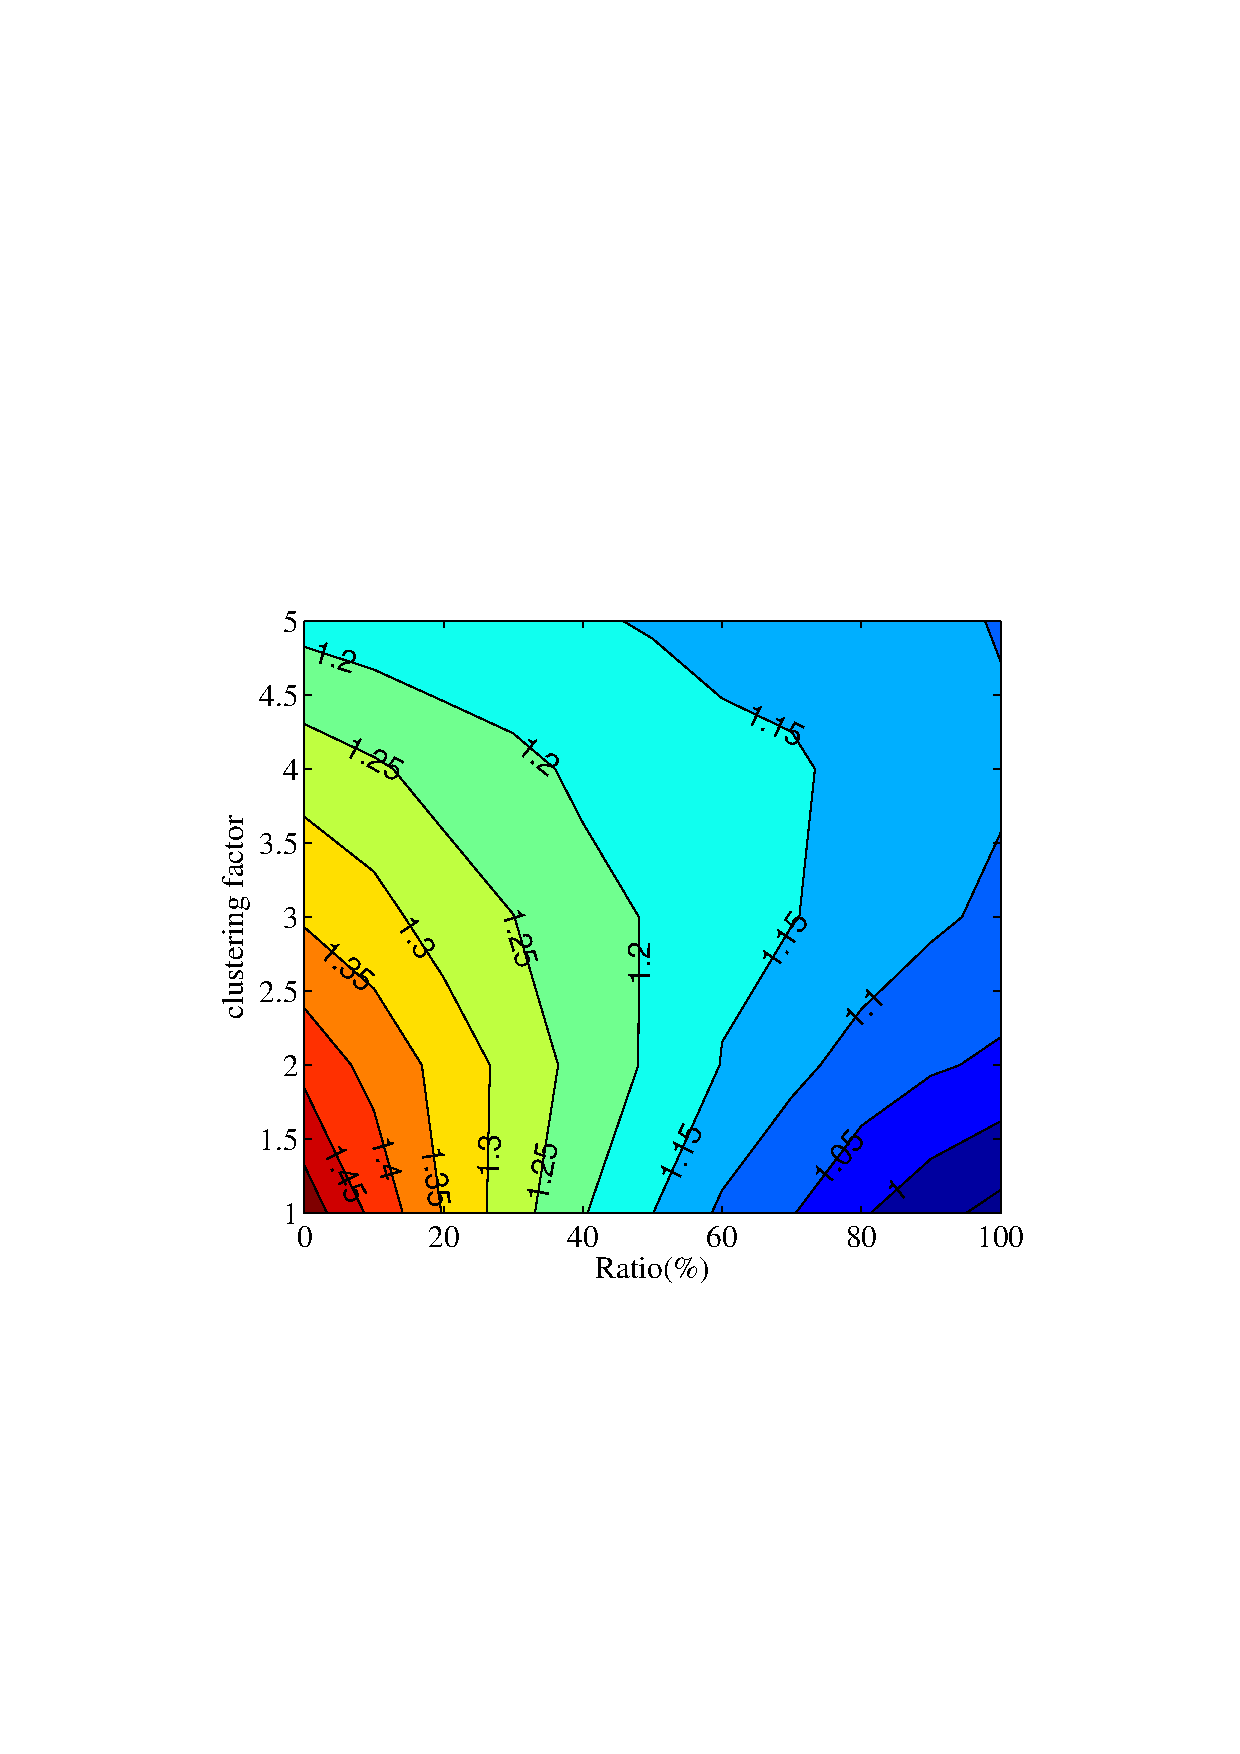
\includegraphics[width=0.8\linewidth]{figure/cfactor.pdf}
	\caption{Experiment 1: Speedup of Horizontal Clustering (HC).}
	\label{fig:shc}
	\vspace{-10pt}
\end{figure}

Experiment 2: Fig.~\ref{fig:performance} (top) shows the performance gain over HC $\mu$ of the balancing methods compared to the HC method for the LIGO workflow. HIFB and HDB significantly increase the performance of the workflow execution. Both strategies capture the structural and runtime information, reducing data transfers between tasks, while HRB focuses on runtime distribution, which in this case is none. Fig.~\ref{fig:performance} (bottom) shows the performance of the balancing methods for the Epigenomics workflow. When increasing the average data size, only HDB demonstrates significantly improvement related to HC. Investigating the structure of the Epigenomics workflow (Fig.~\ref{fig:shape}-bottom), we can see that all tasks at the same horizontal level share the same IFs ($HIFV$ = 0), because each branch (surrounded by dash lines) happen to have the same amount of pipelines. Thus, HIFB has no performance improvement when compared to HC. However, for LIGO (Fig.~\ref{fig:shape}-top), $HIFV \neq 0$, thus HIFB improves the workflow runtime performance.  
%The intuition behind this difference between HDB and HIFB is that 
HDB captures the strong connections between tasks (data dependencies) and HIFB captures the weak connections (similarity in terms of structure). In both workflows, $HDV$ is not zero thus HDB performs better than HC. 

% It is clear that with the increase of the average data size, both HDB and HIFB perform better than HRB. The reason is that both HDB and HIFB can capture the structural information and runtime information, while HRB only focuses on runtime distribution but in this case there is no runtime variance at the horizontal level. 

\begin{figure}[htb]
	\centering
	\includegraphics[width=\linewidth]{figure/exp2_ligo.pdf}
	\includegraphics[width=\linewidth]{figure/exp2_genome.pdf}
	\caption{Experiment 2: Performance of the LIGO workflow (top) and the Epigenomics workflow (bottom).}
	\label{fig:performance}
	\vspace{-10pt}
\end{figure}

Experiment 3: Fig.~\ref{fig:incluence_of_hrv} shows the performance gain $\mu$ when varying task runtimes for the LIGO workflow. As expected, when $HRV$ increases HRB over performs HC. However, HDB and HIFB demonstrate poor performance because they merge tasks based on data dependencies first, and then, they balance the runtime distribution. 
For high values of $HRV$, we just simply need to use HRB. Otherwise, we can use either HDB or HIFB while in some cases HIFB fails to capture the structural information. 

\begin{figure}[htb]
\centering
	\includegraphics[width=\linewidth]{figure/exp3.pdf}
	\caption{Experiment 3: Influence of $HRV$ (LIGO workflow).}
	\label{fig:incluence_of_hrv}
	\vspace{-10pt}
\end{figure}




% Section
\section{Experiments}
\label{sec:experiments}


We applied these imbalance metrics and balanced clustering methods to four widely used workflows in our experiments. We adopt a traced based simulation to evaluate our these metrics and methods. 
We first extended the WorkflowSim~\cite{Chen2012a} simulator with the balanced clustering methods and imbalance metrics to simulate a distributed environment where we could evaluate the performance of our methods when varying the average data size and task runtime. The simulated computing platform is composed by 20 single homogeneous core virtual machines (worker nodes), which is the quota per user of some typical distributed environments such as Amazon EC2~\cite{AmazonAWS} and FutureGrid~\cite{FutureGrid}. Amazon EC2 is a commercial, public cloud that is been widely used in distributed computing. FutureGrid is a distributed, high-performance testbed that provides scientists with a set of computing resources to develop parallel, grid, and cloud applications. We then collected traces of these workflows (including overhead information and task runtime information) from real runs of workflows that were executed on FutureGrid and Amazon EC2. With these traces based information, we use WorkflowSim to vary algorithms used, resources, workflow size etc. to illustrate the different runtime performance of these methods. 

Each simulated VM has 512MB of memory and the capacity to process 1,000 million instructions per second. Task scheduling algorithm is data-aware, i.e. tasks are scheduled to resources which have the most input data available.

The experiments presented hereafter evaluate the performance of our balancing methods in comparison with an existing and effective task clustering strategy named Horizontal Clustering (HC)~\cite{Singh:2008:WTC:1341811.1341822}, which is widely used by workflow management systems such as Pegasus. We also compare our methods with DFJS proposed by Muthuvelu et al.~\cite{Muthuvelu:2005:DJG:1082290.1082297}  that groups bag of tasks based on their runtime—tasks are grouped up to the resource capacity and its extended version AFJS proposed by Liu and Liao~\cite{4958835}, which is an adaptive fine-grained job scheduling algorithm to group fine-grained tasks according to processing capacity and bandwidth of the current available resources. However, DFJS and AFJS requires parameter tuning (resource cap, i.e.) and therefore in this work we use their best performance that is already tuned. In practice, these algorithms are not feasible to use since parameter tuning requires a lot of prior knowledge and it takes much time to search the parameter space without proper heuristics. For example, if the resource capacity is too high, all of the tasks may be grouped together and there is loss of parallelism. If the resource capacity is too low, the algorithms do not group tasks at all, which leads to no improvement over no clustering. For simplicity, we use DFJS* and AFJS* to indicate the best performance of them in the rest of our paper. 

\begin{table*}[!htb]
\caption{Workflow Information }
\label{tab:evaluation_workflows}
\centering
\begin{tabular}{lrrrrrrrr}
\hline
Workflow & Tasks & Avg. Data Size (MB) &  Avg. Task Runtime (secs)  \\

\hline

Epigenomics &165 & 355&2952\\
CyberShake &700&148 & 23\\
LIGO &800& 5&228\\
Montage &300&3 &11\\


\hline
\end{tabular}
\end{table*} 


\begin{figure}[!htb]
	\centering
	\includegraphics[width=0.4\linewidth]{figures/evaluation/inspiral.pdf} \\
	\caption{A simplified visualization of the LIGO Inspiral workflow}
	\label{fig:evaluation_shape_ligo}
\end{figure}

\begin{figure}[htb]
	\centering
	\includegraphics[width=0.6\linewidth]{figures/evaluation/montage.pdf} \\
	\caption{A simplified visualization of the Montage workflow}
	\label{fig:evaluation_shape_montage}
\end{figure}

\begin{figure}[htb]
	\centering
	\includegraphics[width=0.4\linewidth]{figures/evaluation/genome.pdf} \\
	\caption{A simplified visualization of the Epigenomics workflow}
	\label{fig:evaluation_shape_genome}
\end{figure}

\begin{figure}[htb]
	\centering
	\includegraphics[width=0.8\linewidth]{figures/evaluation/cybershake.pdf} \\
	\caption{A simplified visualization of the CyberShake workflow}
	\label{fig:evaluation_shape_cybershake}
\end{figure}


%WorkflowSim is a feature-rich toolkit to simulate workflow planning and execution. It provides runtime randomization and multiple task clustering methods that we need. 

Four workflows are used in the experiments: LIGO~\cite{LIGO} Inspiral analysis, Montage~\cite{Berriman2004}, CyberShake~\cite{Graves2010} and Epigenomics~\cite{Epigenome}. 
%%%

LIGO (Laser Interferometer Gravitational Wave Observatory) workflows are used to search for gravitational wave signatures in data collected by large-scale interferometers. The observatories' mission is to detect and measure gravitational waves predicted by general relativity─Einstein's theory of gravity─in which gravity is described as due to the curvature of the fabric of time and space. LIGO Inspiral workflow is a data intensive workflow. 

CyberShake is a seismology application that calculates Probabilistic Seismic Hazard curves for geographic sites in the Southern California region. It identifies all ruptures within 200km of the site of interest and convert rupture definition into multiple rupture variations with differing hypocenter locations and slip distributions. It then calculates synthetic seismograms for each rupture variance and peak intensity measures are then extracted from these synthetics and combined with the original rupture probabilities to produce probabilistic seismic hazard curves for the site.  


Montage is an astronomy application that is used to construct large image mosaics of the sky. Input images are reprojected onto a sphere and overlap is calculated for each input image. The application re-projects input images to the correct orientation while keeping background emission level constant in all images. The images are added by rectifying them into a common flux scale and background level. Finally the reprojected images are co- added into a final mosaic. The resulting mosaic image can provide a much deeper and detailed understanding of the portion of the sky in question.

The Epigenomics workflow is a pipeline workflow. Initial data are acquired from the Illumina-Solexa Genetic Analyzer in the form of DNA sequence lanes. Each Solexa machine can generate multiple lanes of DNA sequences. These data are converted into a format that can be used by sequence mapping software. The mapping software can do one of two major tasks. It either maps short DNA reads from the sequence data onto a reference genome, or it takes all the short reads, treats them as small pieces in a puzzle and then tries to assemble an entire genome. In our experiments, the workflow maps DNA sequences to the correct locations in a reference Genome. This generates a map that displays the sequence density showing how many times a certain sequence expresses itself on a particular location on the reference genome. Scientists draw conclusions from the density of the acquired sequences on the reference genome. Epigenome is a CPU-intensive application. 

Fig.~\ref{fig:evaluation_shape_ligo},~\ref{fig:evaluation_shape_montage},~\ref{fig:evaluation_shape_genome} and~\ref{fig:evaluation_shape_cybershake} show their simplified workflow structures respectively. For simplicity, we only show one of their branch. 
All of these workflows are generated and varied using the Workflow Generator~\cite{WorkflowGenerator}. Runtime (average and task runtime distribution) and overhead (workflow engine delay, queue delay, and network bandwidth) information were collected from real traces production environments~\cite{Chen2011, Juve2013}, then used as input parameters for the simulations. 

Table~\ref{tab:evaluation_workflows} show their statistical information. 

Three sets of experiments are conducted. 

Experiment 1 evaluates the performance gain over No Clustering ($\mu$) with our balancing methods (HIFB, HDB, HRB) and existing HC, DFJS* and AFJS* algorithms. Since DFJS requires one parameter (resource capacity) and AFJS requires two parameters (resource capacity and bandwidth capacity), we search all possible parameters to use their optimal performance gain. In practice, their performance should be equal to or lower than the optimal values. 

Experiment 2 evaluates the influence of average data size, number of VMs and workflow size (the number of tasks of a workflow) in our balancing methods for one workflow (LIGO). 
%since data has becoming more and more intensive in scientific workflows~\cite{Juve2013}.
The original average data size (both input and output data) of the LIGO workflow is about 5MB as shown in Table~\ref{tab:evaluation_workflows}, and we increase it to 500MB to simulate the case with data intensive workflows. 

Experiment 3 evaluates the influence of combining our horizontal clustering methods with vertical clustering. We compare the performance gain under four scenario, VC-prior: we perform VC first and then HIFB, HDB, HDB or HDC; VC-posterior: we perform horizontal methods and then VC; no VC: horizontal methods only; and VC only. The motivation behind this experiment is that we believe VC will change imbalance metrics (HIFV, HDV and HRV) and we aim to show how these metrics can help us understand the performance of VC better. 

\subsection{Results and Discussion}
\begin{figure}[htb]
	\centering
	\includegraphics[width=0.8\linewidth]{figures/evaluation/big_genome.pdf} \\
	\caption{A visualization of the Epigenomics workflow}
	\label{fig:evaluation_shape_big_genome}
\end{figure}

\begin{figure}[!htb]
	\centering
	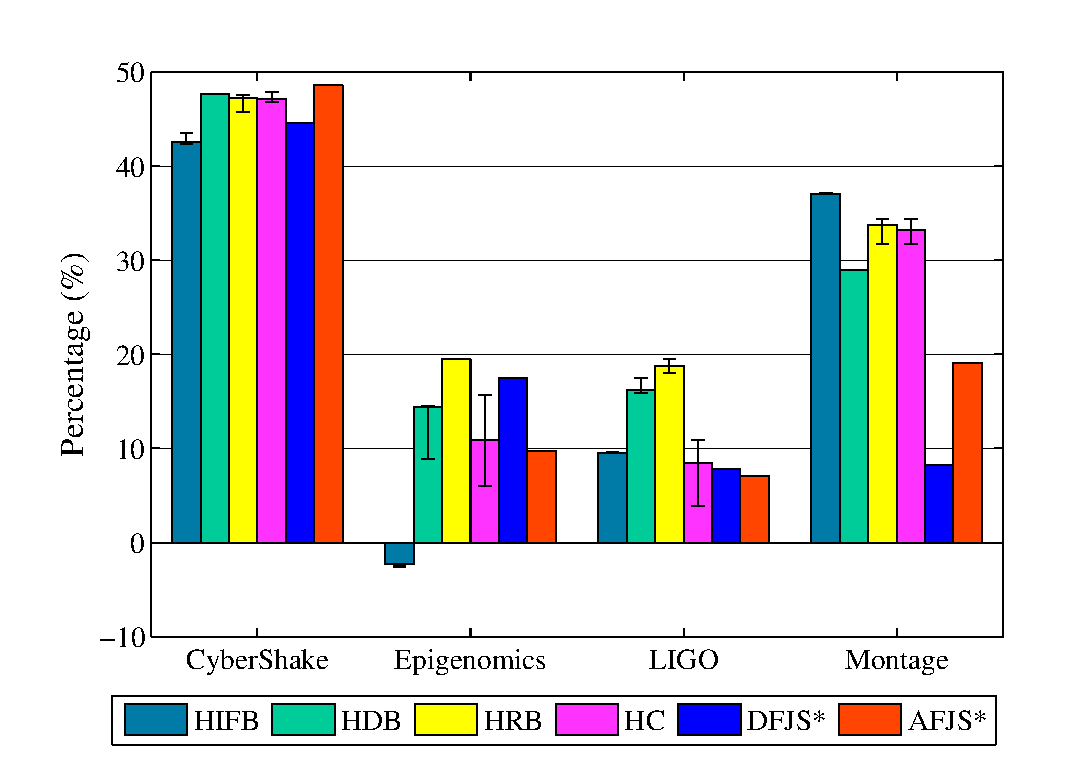
\includegraphics[width=1.0\linewidth]{figures/evaluation/algorithm2.eps}
	\captionof{figure}{Performance Gain over No Clustering of Six Algorithms (* indicates the best performance of DFJS and AFJS)}
	\label{fig:evaluation_algorithm}
\end{figure}

\begin{figure*}[!htb]
	\centering
    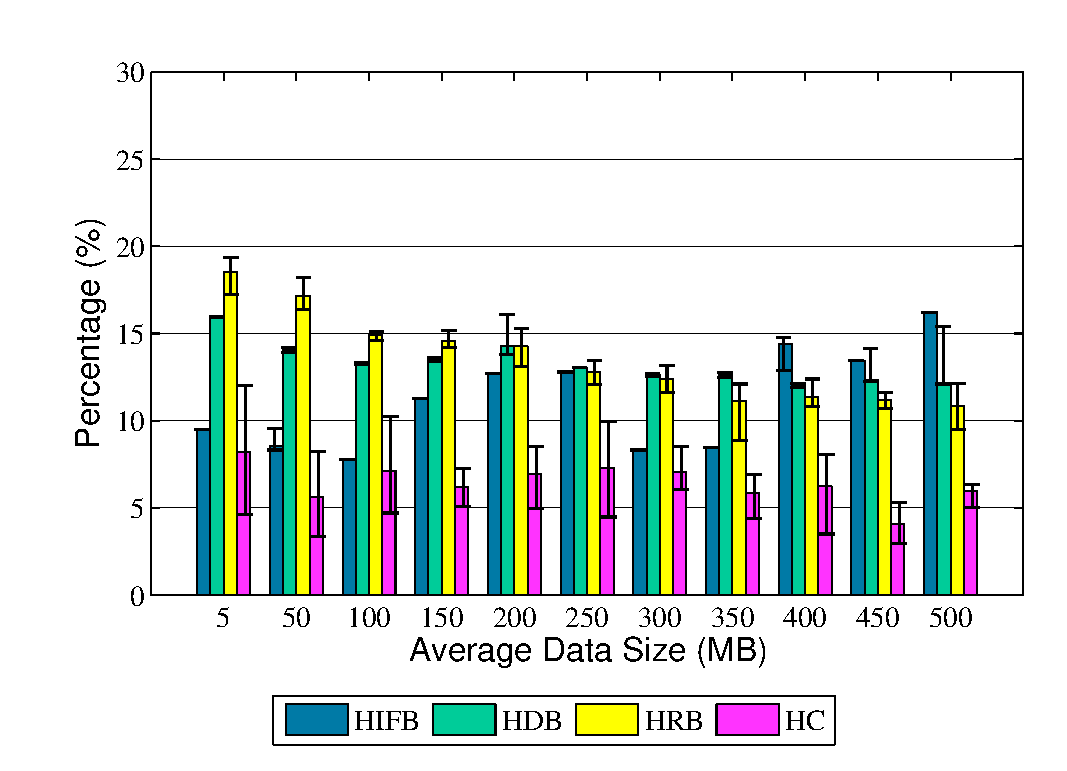
\includegraphics[width=0.7\textwidth]{figures/evaluation/datasize2.eps}
    \caption{Performance Gain over No Clustering with Different Data Size}
    \label{fig:evaluation_datasize}
\end{figure*}

\begin{figure}[!htb]
	\centering
	\includegraphics[width=1.0\linewidth]{figures/evaluation/resource1.eps}
	\captionof{figure}{Performance Gain over No Clustering with Different Number of Resources (Average data size is 5MB).}
	\label{fig:evaluation_resource_1}
\end{figure}

\begin{figure}[!htb]
	\centering
	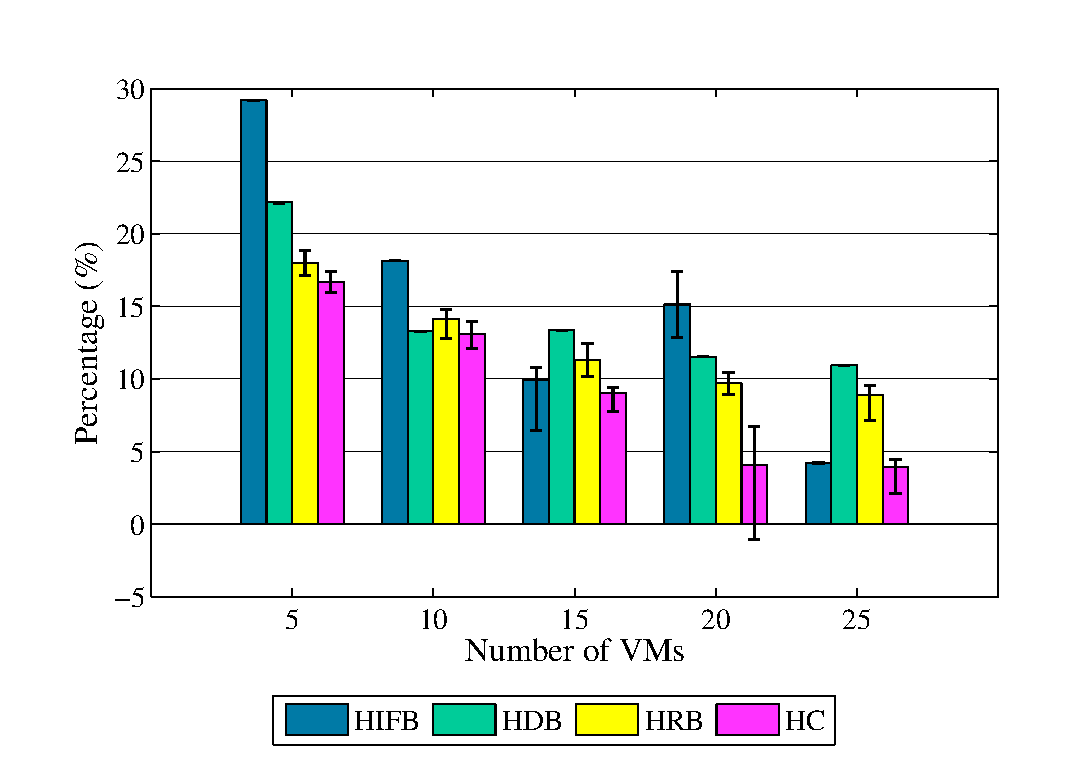
\includegraphics[width=1.0\linewidth]{figures/evaluation/resource2.eps}
	\captionof{figure}{Performance Gain over No Clustering with Different Number of Resources (Average data size is 500MB)).}
	\label{fig:evaluation_resource_2}
\end{figure}
Experiment 1: Fig.~\ref{fig:evaluation_algorithm}  shows the performance gain over No Clustering (NC) $\mu$ of the balancing methods for the four workflows. We have a few conclusions from Fig.~\ref{fig:evaluation_algorithm}: (1). In general, all of these horizontal clustering methods improve the runtime performance significantly (up to 48\%) except for the case using HIFB in Epigenomics. The reason is that each branch of Epigenomics happen to have the same number of pipelines as Fig.~\ref{fig:evaluation_shape_big_genome} shows. In such case, the IFs of each task at the same horizontal level is the same and thus the HIFB cannot distinguish tasks and their dependency variance as shown in Table.~\ref{tab:evaluation_genome}. 
(2). Among the four workflows, we see more significant improvement for the CyberShake workflow and the Montage workflow compared to Epigenomics and LIGO. The reason is Epigenomics and LIGO have a relatively short task runtime compared to the system overheads and task clustering can significantly improve the overall runtime. 
(3). Among the five methods, in most of the cases, it is clear that our methods (HIFB, HDB and HRB) perform better than HC, DFJS* and AFJS*. The reason is that they don't take the runtime variance and dependency variance into consideration. As to the comparison among HIFB, HDB and HRB, we will show in Experiment 2. 

Experiment 2: Fig.~\ref{fig:evaluation_datasize} shows the performance gain of HIFB, HDB, HRB and HC for the LIGO Inspiral workflow. The reason we chose the LIGO Inspiral workflow is that it has most significant difference among these methods. It is clear that with the increase of average data size, HIFB performs better and better while HRB performs worse. We don't see much difference of HC and HDB while varying data size. The reason is HIFB is able to capture the structural and runtime information, reducing data transfers between tasks, while HRB focuses on runtime distribution only. Therefore, while the workflow is more data intensive, we observe better performance of HIFB and a worse performance of HRB. HC does not change much since it is randomly merges tasks at the same horizontal level without information about runtime or data dependency. HDB does not change much since its performance gain is already good enough. 


\begin{figure}[!htb]
	\centering
	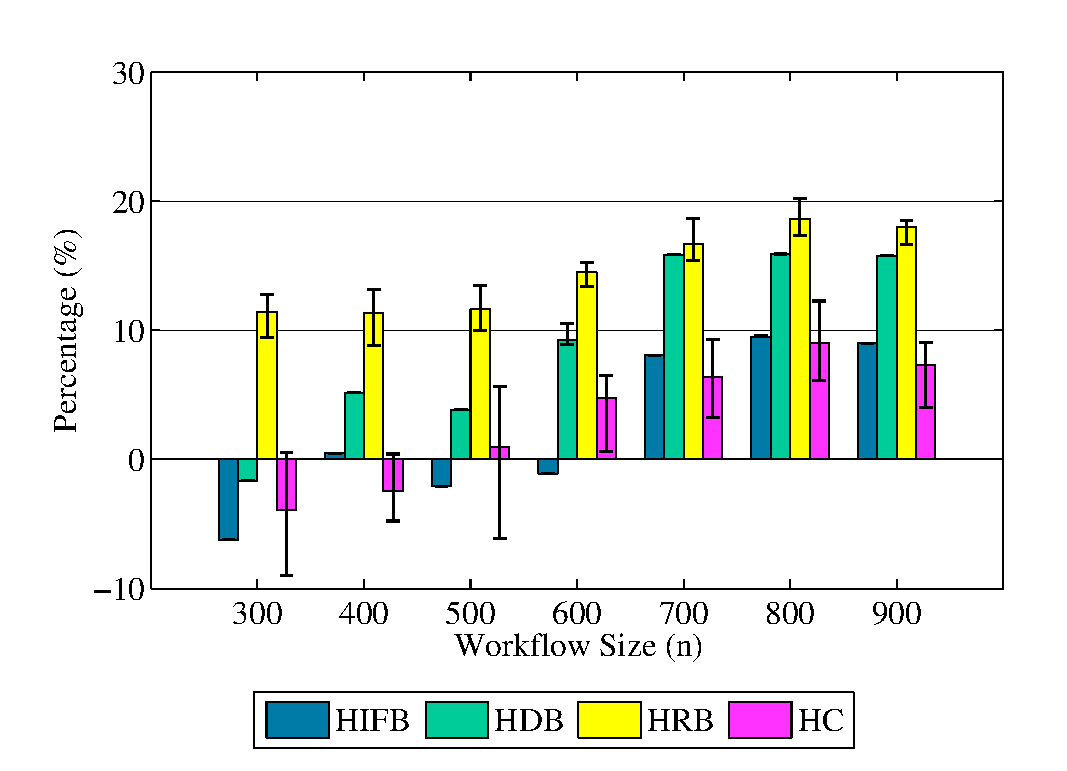
\includegraphics[width=1.0\linewidth]{figures/evaluation/workflowsize.eps}
	\captionof{figure}{Performance Gain over No Clustering with different Workflow Sizes}
	\label{fig:evaluation_wfsize}
\end{figure}

\begin{figure}[!htb]
	\centering
	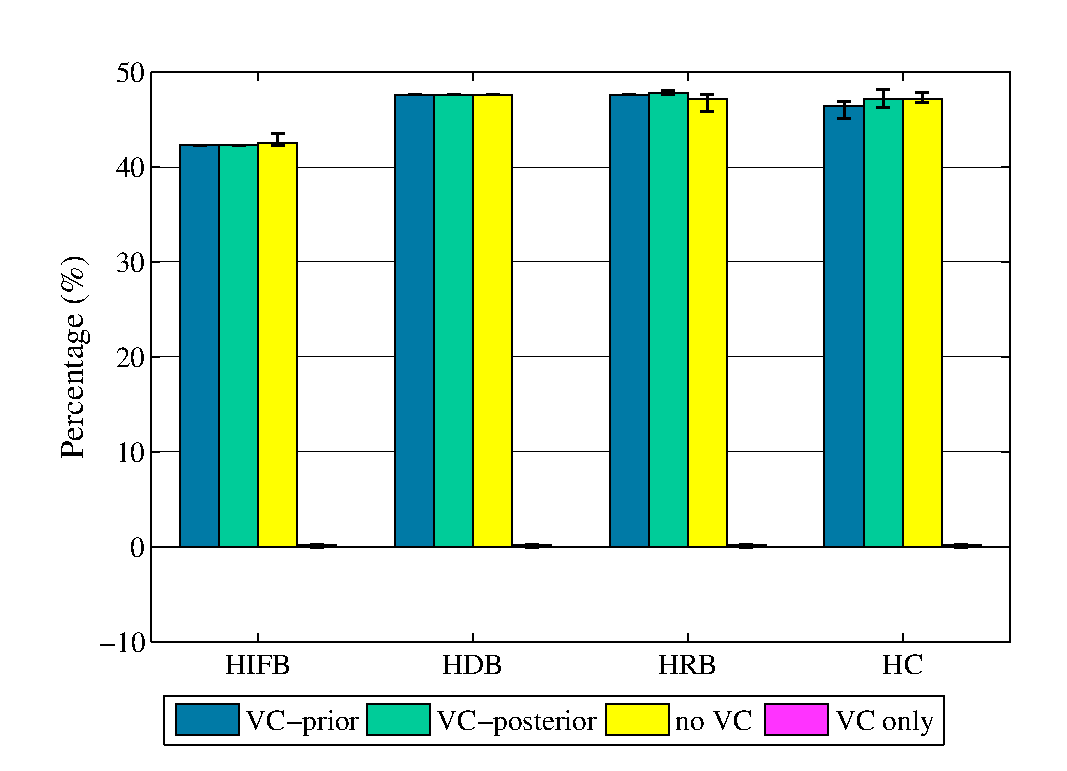
\includegraphics[width=1.0\linewidth]{figures/evaluation/vc_cybershake2.eps}
	\captionof{figure}{Performance Gain over No Clustering for Vertical Methods (CyberShake)}
	\label{fig:evaluation_vc_cybershake}
\end{figure}



\begin{figure}[!htb]
	\centering
    \includegraphics[width=1\linewidth]{figures/evaluation/vc_ligo2.eps}
    \captionof{figure}{Performance Gain over No Clustering for Vertical Methods (LIGO)}
    \label{fig:evaluation_vc_ligo}
\end{figure}


\begin{figure}[!htb]
	\centering
	\includegraphics[width=1.0\linewidth]{figures/evaluation/vc_montage2.eps}
	\captionof{figure}{Performance Gain over No Clustering for Vertical Methods (Montage)}
	\label{fig:evaluation_vc_montage}
\end{figure}

\begin{figure}[!htb]
	\centering
	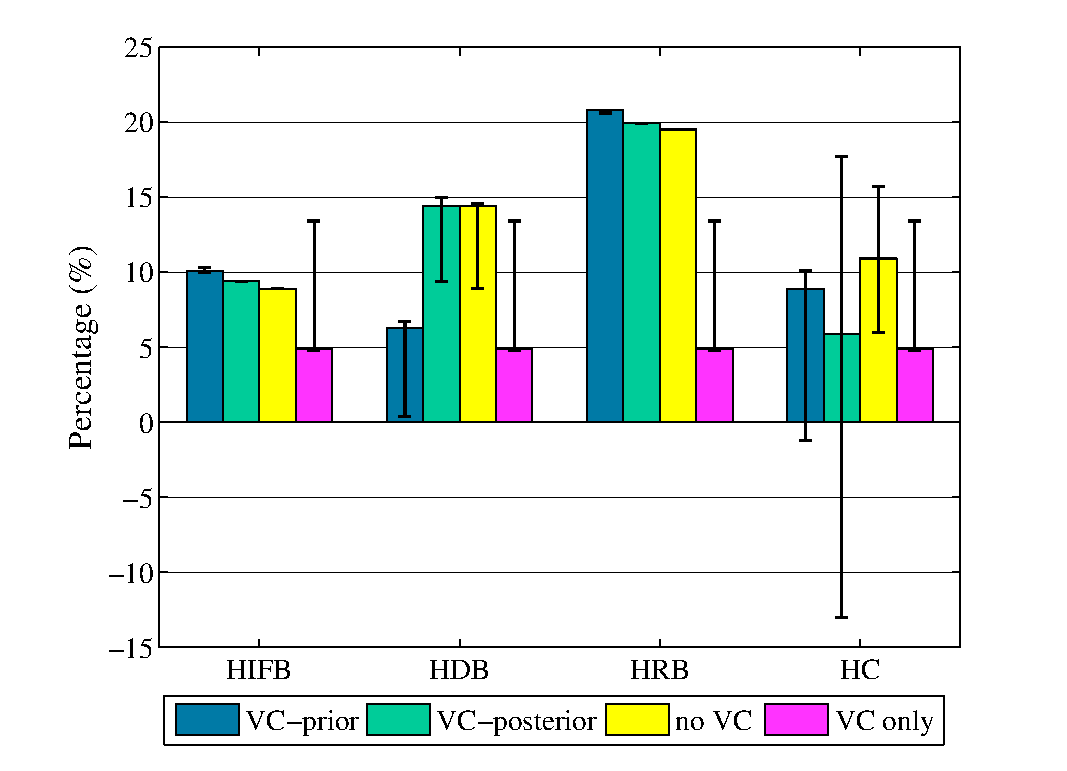
\includegraphics[width=1.0\linewidth]{figures/evaluation/vc_genome2.eps}
	\captionof{figure}{Performance Gain over No Clustering for Vertical Methods (Genome)}
	\label{fig:evaluation_vc_genome}
\end{figure}

\begin{table}[!htb]
\caption{Imbalance Metrics (Montage)}
\label{tab:evaluation_montage}
\centering
\begin{tabular}{lrrrrrrrr}
\hline
Level & Tasks & HRV &  HIFV & HDV  \\

\hline
1 &49 & 0.022 & 0.007 & 189.170 \\
2 & 196 & 0.010 & 0 & 0\\
3 & 1 & 0 & 0 & 0\\
4 & 1 & 0 & 0 & 0\\
5 &49 & 0.017 & 0 & 0\\
6 & 1 & 0 & 0 & 0 \\
7 &1  & 0 & 0 & 0\\
8 &1 & 0 & 0 & 0\\
9 & 1 & 0 & 0 & 0\\
\hline
\end{tabular}
\end{table} 

\begin{table}[!htb]
\caption{Imbalance Metrics (Epigenomics)}
\label{tab:evaluation_genome}
\centering
\begin{tabular}{lrrrrrrrr}
\hline
Level & Tasks & HRV &  HIFV & HDV  \\

\hline
1 & 3 & 0.327 & 0 & 0 \\
2 & 39 & 0.393 & 0 & 578\\
3 & 39 & 0.328 & 0 & 421\\
4 & 39 & 0.358 & 0 & 264\\
5 &39 & 0.290 & 0 & 107\\
6 & 3 & 0.247 & 0 & 0 \\
7 &1  & 0 & 0 & 0\\
8 &1 & 0 & 0 & 0\\
9 & 1 & 0 & 0 & 0\\
\hline
\end{tabular}
\end{table} 

\begin{table}[!htb]
\caption{Imbalance Metrics (CyberShake)}
\label{tab:evaluation_cybershake}
\centering
\begin{tabular}{lrrrrrrrr}
\hline
Level & Tasks & HRV &  HIFV & HDV  \\

\hline
1 & 4 & 0.309 & 0.031 & 1.225 \\
2 & 347 & 0.282 & 0 & 0\\
3 & 348 & 0.397 & 0 & 26.2\\
4 & 1 & 0 & 0 & 0 \\

\hline
\end{tabular}
\end{table} 


\begin{table}[!htb]
\caption{Imbalance Metrics (LIGO)}
\label{tab:evaluation_ligo}
\centering
\begin{tabular}{lrrrrrrrr}
\hline
Level & Tasks & HRV &  HIFV & HDV  \\

\hline
1 & 191 & 0.024 & 0.01 & 10097 \\
2 & 191 & 0.279 & 0.01 & 8264\\
3 & 18 & 0.054 & 0 & 174\\
4 & 191 & 0.066 & 0.01 & 5138\\
5 & 191 & 0.271 & 0.01 & 3306\\
6 & 18 &  0.04 & 0 & 43.7\\

\hline
\end{tabular}
\end{table} 


\begin{table}[!htb]
\caption{Imbalance Metrics (LIGO after performing VC)}
\label{tab:evaluation_ligo_vc}
\centering
\begin{tabular}{lrrrrrrrr}
\hline
Level & Tasks & HRV   \\

\hline
1,2 & 191 & 0.271  \\
3 & 18 & 0.054 \\
4,5 & 191 & 0.268 \\
6 & 18 &  0.04 \\

\hline
\end{tabular}
\end{table} 


Fig.~\ref{fig:evaluation_resource_1} and Fig.~\ref{fig:evaluation_resource_2} vary the number of VMs with an average data size of 5MB and 500MB respectively. We can see that with the increase of VMs, the performance gain of all of these methods decrease while HIFB and HDB decrease more significantly than HRB and HC. The reason is similar to the case of Fig.~\ref{fig:evaluation_datasize} since HIFB and HDB are data dependency aware. The difference between HDB and HIFB is HDB captures the strong connections between tasks (data dependencies) and HIFB captures the weak connections (similarity in terms of structure). In some cases, HIFV is zero (i.e, Epigenomics) while HDV is less unlikely to be zero. Fig.~\ref{fig:evaluation_wfsize} compares the performance gain of these algorithms by varying the workflow sizes (number of tasks in a workflow). By default, the LIGO Inspiral workflow in our paper has 800 tasks. With the decrease of workflow size, we can see that all of these methods perform worse. The reason is there is less resource contention with the decrease of workflow size and therefore task clustering does not perform well. The performance of HRB is more stable since the increase (or decrease) of workflow size has more significant impact on data transfer (roughly linear increase in runtime and square increase in data transfer). 

Experiment 3: Fig.~\ref{fig:evaluation_vc_cybershake},~\ref{fig:evaluation_vc_ligo},~\ref{fig:evaluation_vc_montage} and ~\ref{fig:evaluation_vc_genome} show the performance gain of combining VC along with our horizontal methods with four workflows respectively. For the CyberShake workflow as shown in Fig.~\ref{fig:evaluation_vc_cybershake}, we do not observe any significant change with VC since CyberShake does not have an explicit pipeline that we can perform vertical clustering (the performance gain of VC only is almost zero). 


For the LIGO Inspiral workflow as shown in Fig.~\ref{fig:evaluation_vc_ligo}, we can see that VC-prior perform better than other combination approaches. The reason is VC-prior increases HRV and allows horizontal methods to improve the performance further while VC-posterior does not have many tasks to merge since horizontal methods change the pipeline structures. Table.~\ref{tab:evaluation_ligo_vc} shows the HRV after we perform VC on the LIGO Inspiral workflow. 

For the Montage workflow as shown in Fig.~\ref{fig:evaluation_vc_montage}, we do see significant improvement with VC (about 15\% more than the case without VC). However, the performance improvement does not distinguish these horizontal methods. The reason is tasks merges by VC (the middle and the tail levels of Montage as shown in Fig.\ref{fig:evaluation_shape_montage})are different from the one merged by horizontal methods (the first two levels in Fig.~\ref{fig:evaluation_shape_montage}). Therefore, the performance of VC-posterior and VC-prior does not differ from each other.  


For the Epigenomics workflow as shown in Fig.~\ref{fig:evaluation_vc_genome}, we observe similar phenomenon in HRB compared to the LIGO Inspiral workflow. As to the performance of HDB, VC-prior merges tasks at the second, third, fourth and fifth level together and thus HDB has less space to further improve the overall runtime. 
 
%HIFB and HDB significantly increase the performance of the workflow execution. Both strategies capture the structural and runtime information, reducing data transfers between tasks, while HRB focuses on runtime distribution, which in this case is none. Fig.~\ref{fig:imbalance_performance} (bottom) shows the performance of the balancing methods for the Epigenomics workflow. When increasing the average data size, only HDB demonstrates significantly improvement related to HC. Investigating the structure of the Epigenomics workflow (Fig.~\ref{fig:imbalance_shape}-bottom), we can see that all tasks at the same horizontal level share the same IFs ($HIFV$ = 0), because each branch (surrounded by dash lines) happen to have the same amount of pipelines. Thus, HIFB has no performance improvement when compared to HC. However, for LIGO (Fig.~\ref{fig:imbalance_shape}-top), $HIFV \neq 0$, thus HIFB improves the workflow runtime performance.  
%The intuition behind this difference between HDB and HIFB is that 
%HDB captures the strong connections between tasks (data dependencies) and HIFB captures the weak connections (similarity in terms of structure). In both workflows, $HDV$ is not zero thus HDB performs better than HC. 







\section{Conclusion and Future Work}

We presented three balancing methods and two vertical clustering combination approaches to address the load balance problem when clustering workfl�ow tasks. We also defi�ned three imbalance metrics to quantitatively measure workfl�ow characteristics based on task runtime variation (HRV), task impact factor (HIFV), and task distance variance (HDV).

Three experiment sets were conducted using traces from five real workflow applications. The first experiment aimed at measuring the performance gain over a baseline execution without clustering. In addition, we compared our balancing methods with three algorithms in literature. Experimental results show that our methods yield significant improvement over a baseline execution, and that they have acceptable performance when compared to the best estimated performance of the existing algorithms. The second experiment measured the influence of average data size and number of available resources on the performance gain. In particular, results show that our methods have different sensitivity to data- and computational-intensive workflows. Finally, the last experiment evaluated the interest of performing horizontal and vertical clustering in the same workflow. Results show that vertical clustering can significantly improve pipeline-structured workflows, but it is not suitable if the workflow has no explicit pipelines.

The simulation based evaluation also shows that the performance improvement of the proposed balancing algorithms (HRB, HDB and HIFB) is highly related to the metric values (HRV, HDV and HIFV) that we introduced. For example, a workflow with high HRV tends to have better performance improvement with HRB since HRB is used to balance the runtime variance. 

In the future, we plan to further analyze the imbalance metrics proposed. For instance, the values of these metrics presented in this paper are not normalized, and thus their values per level (HIFV, HDV, and HRV) are in different scales. Also, we plan to analyze more workflow applications, particularly the ones with asymmetric structures, to investigate the relationship between workflow structures and the metric values. 

Also, as shown in Figure~\ref{fig:evaluation_vc_genome}, \emph{VC-prior} can generate very large clustered jobs vertically and makes it difficult for horizontal methods to improve further. Therefore, we aim to develop imbalance metrics for \emph{VC-prior} to avoid generating large clustered jobs, i.e., based on the accumulated runtime of tasks in a pipeline. 


As shown in our experiment results, the combination of our balancing methods with vertical clustering have different sensitivity to workflows with distinguished graph structures and runtime distribution. Therefore, a possible future work is the development of a portfolio clustering, which chooses multiple clustering algorithms, and dynamically selects most suitable one according to the dynamic load.

In this paper, we demonstrate the performance gain of combining horizontal clustering methods and vertical clustering. We plan to combine multiple algorithms together instead of just two. We will develop a policy engine that iteratively chooses one algorithm from all of the balancing methods based on the imbalance metrics until the performance gain converges. 

Finally, we aim at applying our metrics to other workflow study areas, such as workflow scheduling where heuristics would either look into the characteristics of the task when it is ready to schedule (local scheduling), or examine the entire workflow (global optimization algorithms). In this work, the impact factor metric only uses a family of tasks that are tightly related or similar to each other. This method represents a new approach to solve the existing problems. 

\section{Acknowledgements}
This work is funded by NSF IIS-0905032 and NSF FutureGrid 0910812. We thank Gideon Juve, Karan Vahi, Rajiv Mayani, and Mats Rynge for their help. 





%% References with bibTeX database:

\bibliographystyle{elsarticle-num}
\bibliography{biblio}

\end{document}